\subsubsection{\texorpdfstring{\textbf{~1.检错编码}}{~1.检错编码}}\label{ux68c0ux9519ux7f16ux7801}

~ ~
~通过一定的编码和解码,能够在接收端解码时检查出传输的错误,但不能纠正错误。常见的检错编码有奇偶校验码和循环冗余码(CRC)。\emph{}

\textbf{~ ~
~1)奇(偶)校验码。}添加一位校验码后,使得整个码字里面1的个数是奇(偶)数。接收端收到数据后就校验一下数据里1的个数,如果正好为奇(偶)数,则认为传输没有出错;如果检测到偶(奇)数个1,则说明传输过程中,数据发生了改变,要求重发。

\textbf{~ ~
注意:}当数据中有一位数据发生改变,通过奇偶校验能够检测出来,但并不知道是哪个位出错了;如果数据中同时有两位数发生了改变,此时奇偶校验是检测不到数据出错的,所以它的查错能力有限。\textbf{}

\textbf{~ ~ ~ ~ ~
~2)循环冗余码。}循环冗余校验码是通过除法运算来建立有效信息位和校验位之间的约定关系。假定,待编码的有效信息以多项式M(x)表示,将它左移若干位后,用另一个约定的多项式G(x)去除,所产生的余数就是校验位。有效信息位与校验位相拼接就构成了CRC码,如图3-3所示。当接收方收到发来的CRC码后,仍用约定的多项式G(x)去除,若余数为0,表明该代码接收无误;若余数不为0,表明某一位出错,再进一步由余数值确定出错的位置,并予以纠正。

\textbf{~~~~~~~
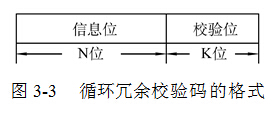
\includegraphics[width=1.20833in,height=1.20833in]{png-jpeg-pics/edd5db9057ecf31dc1c9430401a1e6f1?}}

\textbf{}

\textbf{\textbf{2.纠错编码}}

\textbf{~ ~
就是在接收端不但能检查错误,而且能纠正检查出来的错误。常见的纠错编码是海明码。海明码又称为汉明码,它是在信息字段中插入若干位数据,用于监督码字里的哪一位数据发生了变化,\textbf{具有一位纠错能力}。}

\textbf{\textbf{~ ~(1)海明码的编码过程}}

\textbf{\includegraphics[width=2.08333in,height=2.08333in]{png-jpeg-pics/780c02e6761c557a1ad61d7a253175f6?}\\
\hspace*{0.333em}}{}
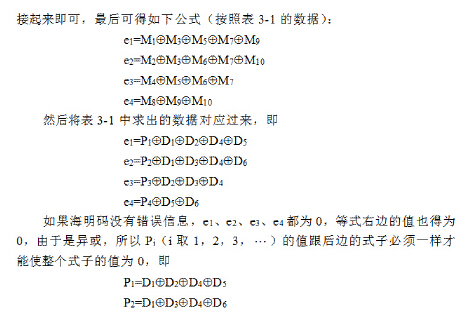
\includegraphics[width=2.08333in,height=2.08333in]{png-jpeg-pics/16c92a7deb65bc0148a582696847fdf0?}\textbf{\\
\hspace*{0.333em}}

\textbf{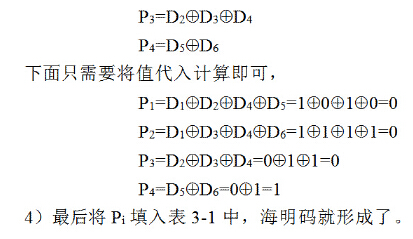
\includegraphics[width=2.08333in,height=2.08333in]{png-jpeg-pics/2f68ce241ce2f12bf140b0ca12311061?}}

\textbf{}

\textbf{\textbf{~ (2)校验海明码的过程}}

\textbf{\\
}{}

\textbf{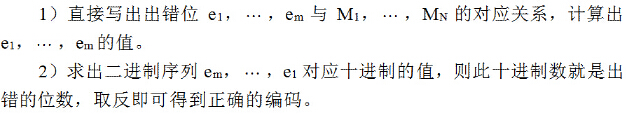
\includegraphics[width=2.08333in,height=2.08333in]{png-jpeg-pics/57a590df95bea387e841aa233c2946d6?}}
